\section{}
The gage pressure of the air in the tank shown in the figure below is
measured to be 50 kPa. Determine the differential height h of the mercury column.

\begin{figure}[h]
    \centering
    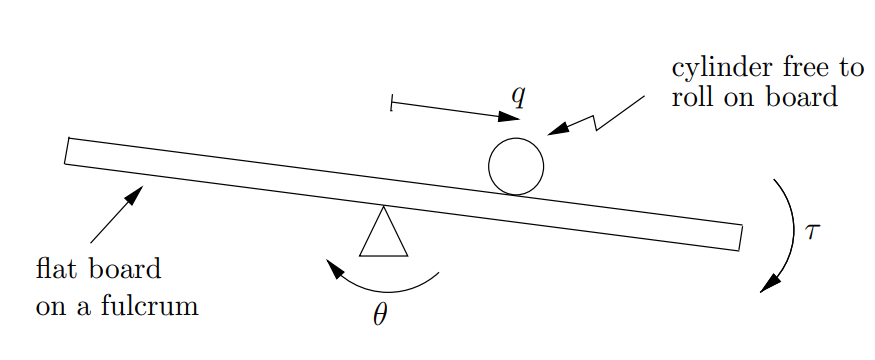
\includegraphics[width=0.5\textwidth]{Questions/Figures/Q4ProblemDiagram.png}
    \caption{Monometer with multiple fluids}
    \label{fig:Q4 System}
\end{figure}

The pressure balance for the system is given by:
\begin{align}
    P_{gauge, air} = P_{w} 
